\documentclass[12pt,letterpaper]{article}

\usepackage{amsmath, amsthm}
\usepackage{graphicx}
\usepackage{microtype, parskip}
\usepackage{caption, subcaption, multirow, morefloats, rotating, longtable}
\usepackage{hyperref}
\usepackage[numbers,sort&compress]{natbib}
\usepackage{authblk, attrib, fullpage}
\usepackage{lineno}


\begin{document}
\setcounter{secnumdepth}{0}

\begin{titlepage}
  \begin{center}
    \huge{Evolutionary paleoecology and the biology of extinction}

    \vspace{1.5cm}

    \large{Peter D. Smits \\}
    \footnotesize{\href{mailto:psmits@uchicago.edu}{psmits@uchicago.edu}}

    \vspace{1.5cm}

    Dissertation Proposal Hearing \\
    \today \\
    Commmittee on Evolutionary Biology \\
    The University of Chicago

    \vspace{1.5cm}

    \textit{Committee} \\
    Dr. Michael J. Foote (co-advisor) \\
    Dr. Kenneth D. Angielczyk (co-advisor) \\
    Dr. Richard H. Ree \\
    Dr. P. David Polly
  \end{center}
\end{titlepage}

\linenumbers
\modulolinenumbers[2]


\section{Introduction and Theory}
Paleobiology is the study of life over time and the inference of what processes generate the observed patterns in diversity and disparity. Intimately related to paleobiology is the concept of macroevolution here defined as the pattern of speciation and extinction over time \citep{Jablonski2008a}. The study of macroevolution is the estimation of the processes underlying these observed patterns. The term origination is frequently used in place of speciation because it includes both speciation and migration and depending on both the spatial scale and quality of the fossil record it may be impossible to distinguish between the two.

Evolutionary paleoecology is defined as the study of the effects of ecological traits and factors on differential rate dynamics, particularly rates of faunal turnover and diversification \citep{Kitchell1985a}. Ecological traits and factors are traits expressed by a taxon, at any level, that are involved with biotic--biotic or biotic--abiotic interactions. Diversification is the difference between origination and extinction and is the net pattern of macroevolution. The study of evolutionary paleoecology is therefore the link between environmental (biotic--biotic and biotic--abiotic) interactions and macroevolution. As a corollary to \citet{Kitchell1985a}'s definition, \citet{Allmon1994} states that in order to correctly link ecological interactions to macroevolution, one must focus on the specific traits and factors that may affect the speciation process. Tacitly included in this is the study of how ecological traits are related to extinction \citep{Kitchell1990}.

It is under this framework that I propose to study how ecological traits associated with environmental preference have affected both the cosmopolitan-endemism dynamics and differential survival. I will be studying two distantly related and biotically different groups: Cenozoic mammals and Permian brachiopods. Both of these groups are considered to have very good fossil records able to reflect massive long term evolutionary patterns \citep{Mark1977}. These two time periods were chosen because they represent periods of climatic change, global cooling and global warming respectively. Also, these two groups are a terrestrial and marine system respectively and the ecological traits associated with range size (described below) are fundamentally very different. 

Survival can be considered the fundamental measure of fitness or evolutionary success because ultimately, a successful lineage is not one that speciated greatly but one that never went extinct \citep{Cooper1984,Palmer2012}. Because during periods of background extinction, extinction is most likely non-random with respect to biology \citep{Jablonski1986}, it should be possible to estimate how various ecological traits affect relative fitness \citep{Kitchell1990,Kitchell1985a}. Periods of background extinction also represent the majority of geologic time. Additionally, these conditions remain predictable and likely to change slowly, thus providing a better opportunity to study how traits affect survival than during mass extinctions \citep{Jablonski1986,Raup1988}.

The relationship between geographic range and extinction risk is well understood. Species with larger geographic ranges tend to have lower extinction rates than species with smaller geographic ranges \citep{Jablonski1986,Harnik2013,Nurnberg2013a,Jablonski2003,Roy2009c}. Range size is considered emergent because no one property of an organism can explain this trait and instead it is a combination of multiple properties which determines range size. However the effect of various organismal traits, such as body size or environmental preference, remains much less well understood. It has been shown that ecological traits can be related to differential extinction \citep{Foote2013,Liow2007b,Baumiller1993,Nurnberg2013a}, especially the relationship of adaptation to variable environments and increased species longevity. While some research has focused on the indirect effect of organismal traits on longevity \citep{Harnik2011}, the interaction between organismal traits and its relationship to survival remains understudied especially during periods of background extinction. Here I propose to study the individual and combined effects of organismal traits related to range size on extinction.


\section{Dynamics of community connectedness in Cenozoic mammals}

\textit{Questions:} 
How does the relationship between endemic and cosmopolitan taxa in average community composition change over time? Is there a single global pattern, or do different continents have different patterns? Do patterns differ between ecological categories? Is global climate change an important predictor of these patterns?

\textit{Background and Predictions:}
Community connectedness is the degree to which localities are composed of endemic versus cosmopolitan taxa, and how similar this ratio is between all localities. How community composition changes over time and in relation to organismal traits as well as a changing environment is extremely important for understanding how trophic structure changes or is maintained. In mammals, two important ecological traits in determining range size and distribution of taxa are dietary category and locomotor category \citep{Jernvall2004,Lyons2005,Lyons2010}. Different dietary categories acts as a limit on abundance because of the available environmental energy or resources in a location \citep{VanValen1989,Brown1987,Damuth1979,Silva1997,Janis2000}. Abundance is correlated with occupancy, or the number of unique localities at which a taxon is found \citep{Jernvall2002,Fortelius2002,Brown1984}. It follows then that limits imposed by environmental energy on abundance would then affect the (possible) range size of a taxon. Locomotor category describes the motility of a taxon and the plausibility of occurrence. Locomotor category also limits the dispersal ability of a taxon. For example, an obligate arboreal taxon can only occur in locations with a minimum of tree cover and can most likely only disperse to other environments with suitable tree cover. Dispersal ability is considered important in determining the extent of a taxon's geographic range \citep{Birand2012,Jablonski2006a,Gaston2009} and thus any trait that would limit the ability for an organism to disperse would most likely limit the range size of that organism.

During the Cenozoic there was a global shift from predominately closed, forested habitat to more open, savanna-like habitat. It is expected that there was an increase in relative endemism of arboreal taxa over time and a decrease in relative endemism of terrestrial taxa. The timing of this environmental shift was different between continents \citep{Stromberg2005,Stromberg2013}, so the patterns of community connectedness may not be globally uniform and could reflect regional differences. Shifts in distribution of taxa by locomotor category may not necessarily accompanied by shifts in distribution related to dietary category, though previous studies are limited and qualitative \citep{Janis1993a}. 

A global trend during the Cenzoic was the shift from a ``hot house'' environment with no polar ice caps to an ``ice house'' environment with polar ice caps \citep{Zachos2008,Zachos2001}. This transition was known to have caused major shifts in the global climatic envelopes and the reorganization of communities along with it \citep{Janis1993a,Fortelius2002,Blois2009,Alroy2000g,Figueirido2012}. For mammalian community connectedness there are two possible scenarios. First, it could be possible that while the environment was shifting, lineages may have adapted in place and overall trophic structure and biogeographic structure remained rather constant through time \citep{Jernvall2004}. Alternatively, species may have shifted ranges and thus changed the set of possible interacting taxa which would be associated with changes in trophic structure as well as community connectedness.

The majority of previous research on mammalian faunal dynamics has focused on the North American fossil record and the effects of climate change on diversity and distribution \citep{Alroy2000g,Alroy1996a,Alroy1998,Barnosky2001a,Simpson1944,Simpson1953,Badgley2013,Blois2009,Figueirido2012,Gunnell1995,Hadly2001}. The long term effects of climate change on North American mammalian diversity dynamics and community connectedness remains unresolved and controversial \citep{Alroy2000g,Blois2009,Figueirido2012,Barnosky2001a}. The basic predictions are that over the Cenozoic there would have been a relative increase in endemism in arboreal taxa versus a relative decrease in endmemism in ground dwelling taxa. Because of the vast amount of prior work on North American mammalian faunal dynamics, this forms the basis for the global predictions made above and the North American record becomes the baseline for comparison with other regions.

The European mammalian fossil record is less studied compared to North America and research has focused primarily on faunal dynamics in the Neogene \citep{Jernvall2002,Jernvall2004,Liow2008,Raia2006,Raia2005,Raia2011c}. One of the major findings is that there was very little shift in relative dietary category abundance \citep{Jernvall2004} while the patterns within herbivores (browse--graze transition) were mostly driven by abundant, cosmopolitan taxa \citep{Jernvall2002}. Because of this, the major predictions for the European record is that occupancy will increase for herbivorous taxa, while increasing or remaining constant in carnivores, and remaining relatively constant or random for omnivores. These different predictions for each of the dietary categories is based on the differences in resilience and relationship with primary productivity, with herbivores being more resilient than carnivores and omnivores being random in their resilience \citep{Jernvall2004}. 

The biogeographic pattens of Cenozoic South American mammalian fauna are unstudied in all but qualitative forms. This lack of information is due to historical reasons, with the fossil record of southern continents being in general under studied compared to that of northern continents. Recently, there has been a dramatic increase in the amount of fossil collecting and coverage of most of the Cenozoic \citep{Macfadden1997,Macfadden2006,Flynn1998a}. Because of this, it should be possible to analyze quantitativly the biogeographic structure of the South American mammal fossil record. The South American mammalian faunal record reflects two distinct biotic provinces between the North and the South \citep{Macfadden1997,Macfadden2006,Flynn1998a,Patterson1968}. Because of this, the South American record is expected to have a different pattern of community connectedness than either North America or Europe. Also, there is an expected increase in land-dwelling herbivores relative to arboreal.


\textit{Proposed research:}
Using methods first proposed by \citet{Sidor2013} and \citet{Vilhena2013}, I propose to construct bipartite biogeographic networks between taxa and localities. Here taxa are defined as species and localities are defined as 2x2 grid cells of an equal-area map projection. Networks will be made for every 2 million year bin of the Cenozoic. This bin width is chosen to have minimum two localities be present in every bin. Additionally, networks will be constructed for each dietary and locomotor category. Previous studies of mammalian occurrence patters have restricted analysis to major orders, such as Primates and Artiodactyls, in order to account for apparent sampling and taxonomic biases. Here, analysis will be done using all available taxa and with a restricted sample of just major orders in order to observe any differences in community connectedness.

Community connectedness will be measured using four summary statistics \citep{Sidor2013}: average relative number of endemics, average relative occupancy, biogeographic connectedness, and code length. The average relative number of endemics is defined as 
%\begin{equation}
\(
  E = \frac{\sum_{i = 1}^{L} \frac{u_{i}}{n_{i}}}{L}
\)
%  \label{eq:end}
%\end{equation}
where \(L\) is as the number of localities, \(u\) is the number of taxa unique to a locality, and \(n\) is the number of taxa present at a locality. This is a measure of how unique localities are. Average relative occupancy is the number of localities a taxon is, on average, found at. It is defined as 
%\begin{equation}
\(
  Occ = \frac{\sum_{i = 1}^{N} \frac{l_{i}}{L}}{N}
\)
%  \label{eq:occ}
%\end{equation}
where \(N\) is as the number of taxa present in the biogeographic network and \(l\) is the number of localities a taxon occurred in. Biogeographic connectedness is a measurement of the shared taxa between localities and is defined as 
%\begin{equation}
\(
  BC = \frac{O - N}{LN - N}
\)
%  \label{eq:bc}
%\end{equation}
where \(O\) is the total number of taxonomic occurrences. \(BC\) ranges from 0 to 1, with 0 meaning that each locality completely disconnected from all other localities and 1 indicating all that taxa shared between all localities. Importantly, \(BC\) is infinite when there is only one locality.

Code length is a measurement of the compressibility and information flow of a graph and is estimated via the map equation \citep{Rosvall2008,Rosvall2010b}. The logic of the map equation is that a good map compresses reality into a few simple symbols. This means we want to compress each section of a graph into individual single symbol. A network with a low code length can be compressed into more distinct subunits/provinces compared to a network than a large code length. In the case of measuring community connectedness, a low code length means greater provinciality than a high code length \citep{Sidor2013}. 

Phylogenetic similarity between localities may play an important role in community structuring \citep{Webb2002}. As such, average phylogenetic similarity will be estimated between all localities during a time bin. As a preliminary approach, for every pairwise combination of localities an informal phylogeny will be constructed for the pool of all taxa present in both localities. This informal phylogeny will be based solely on available taxonomic information such as order, family, and genus assignments. The average patristic distance between all taxa will then be estimated. The average of all pairwise comparisons per bin can then be used in partial correlations and modeling questions for understanding what best explain patterns of community connectedness.

The next step is to compare patterns of community connectedness both within and between regions in order to understand if there is a single global trend or if regional processes dominate as well as comparisons of the different dietary and locomotor categories for similarity within and between traits and regions. The approach and methodology to accomplish this analysis is currently under development. 
%In order to compare whether patterns observed on different continents are similar or different, as well as compare patterns between different categories of ecological traits, HOW DO I DO THIS?

Taxonomic occurrence data will be collected through a combination of the Paleobiology Database (PBDB; \url{http://fossilworks.org}), Neogene Old World Database (NOW; \url{http://www.helsink.fi/science/now/}), and museum collections. North American fossil mammal data is very well represented and vetted in the PBDB because of the extensive work of Alroy \citep{Alroy1996a,Alroy1998,Alroy2000g}. European fossil mammal data is also well represented between the PBDB and NOW. South American fossil mammal data is available through the PBDB, but is not particularly well vetted and has poor overall coverage. Because of this, South American fossil mammal data will be gathered via various museums such as the Field Museum of Natural History and the American Museum of Natural History. With the South American taxa, taxonomy and sampling may not be as well resolved as for North and South America and it may be necessary to restrict analysis to the most taxonomically resolved and sampled groups such as Notoungulata, Marsupials, Carnivora, and Primates.


\textit{Preliminary results}
Preliminary results of the community connectedness patterns of both North America and Europe based on PBDB data are presented here (Fig. \ref{fig:mam_tot}). Both regions have qualitatively very different patterns of community connectedness, primarily in the early Cenozoic. However, almost all four of the network statistics are extremely volatile over the Cenozoic, especially for the European record. However, there some interesting qualitative patterns as illustrated by the generalized additive model smooths.

\begin{figure}[ht]
  \begin{center}
    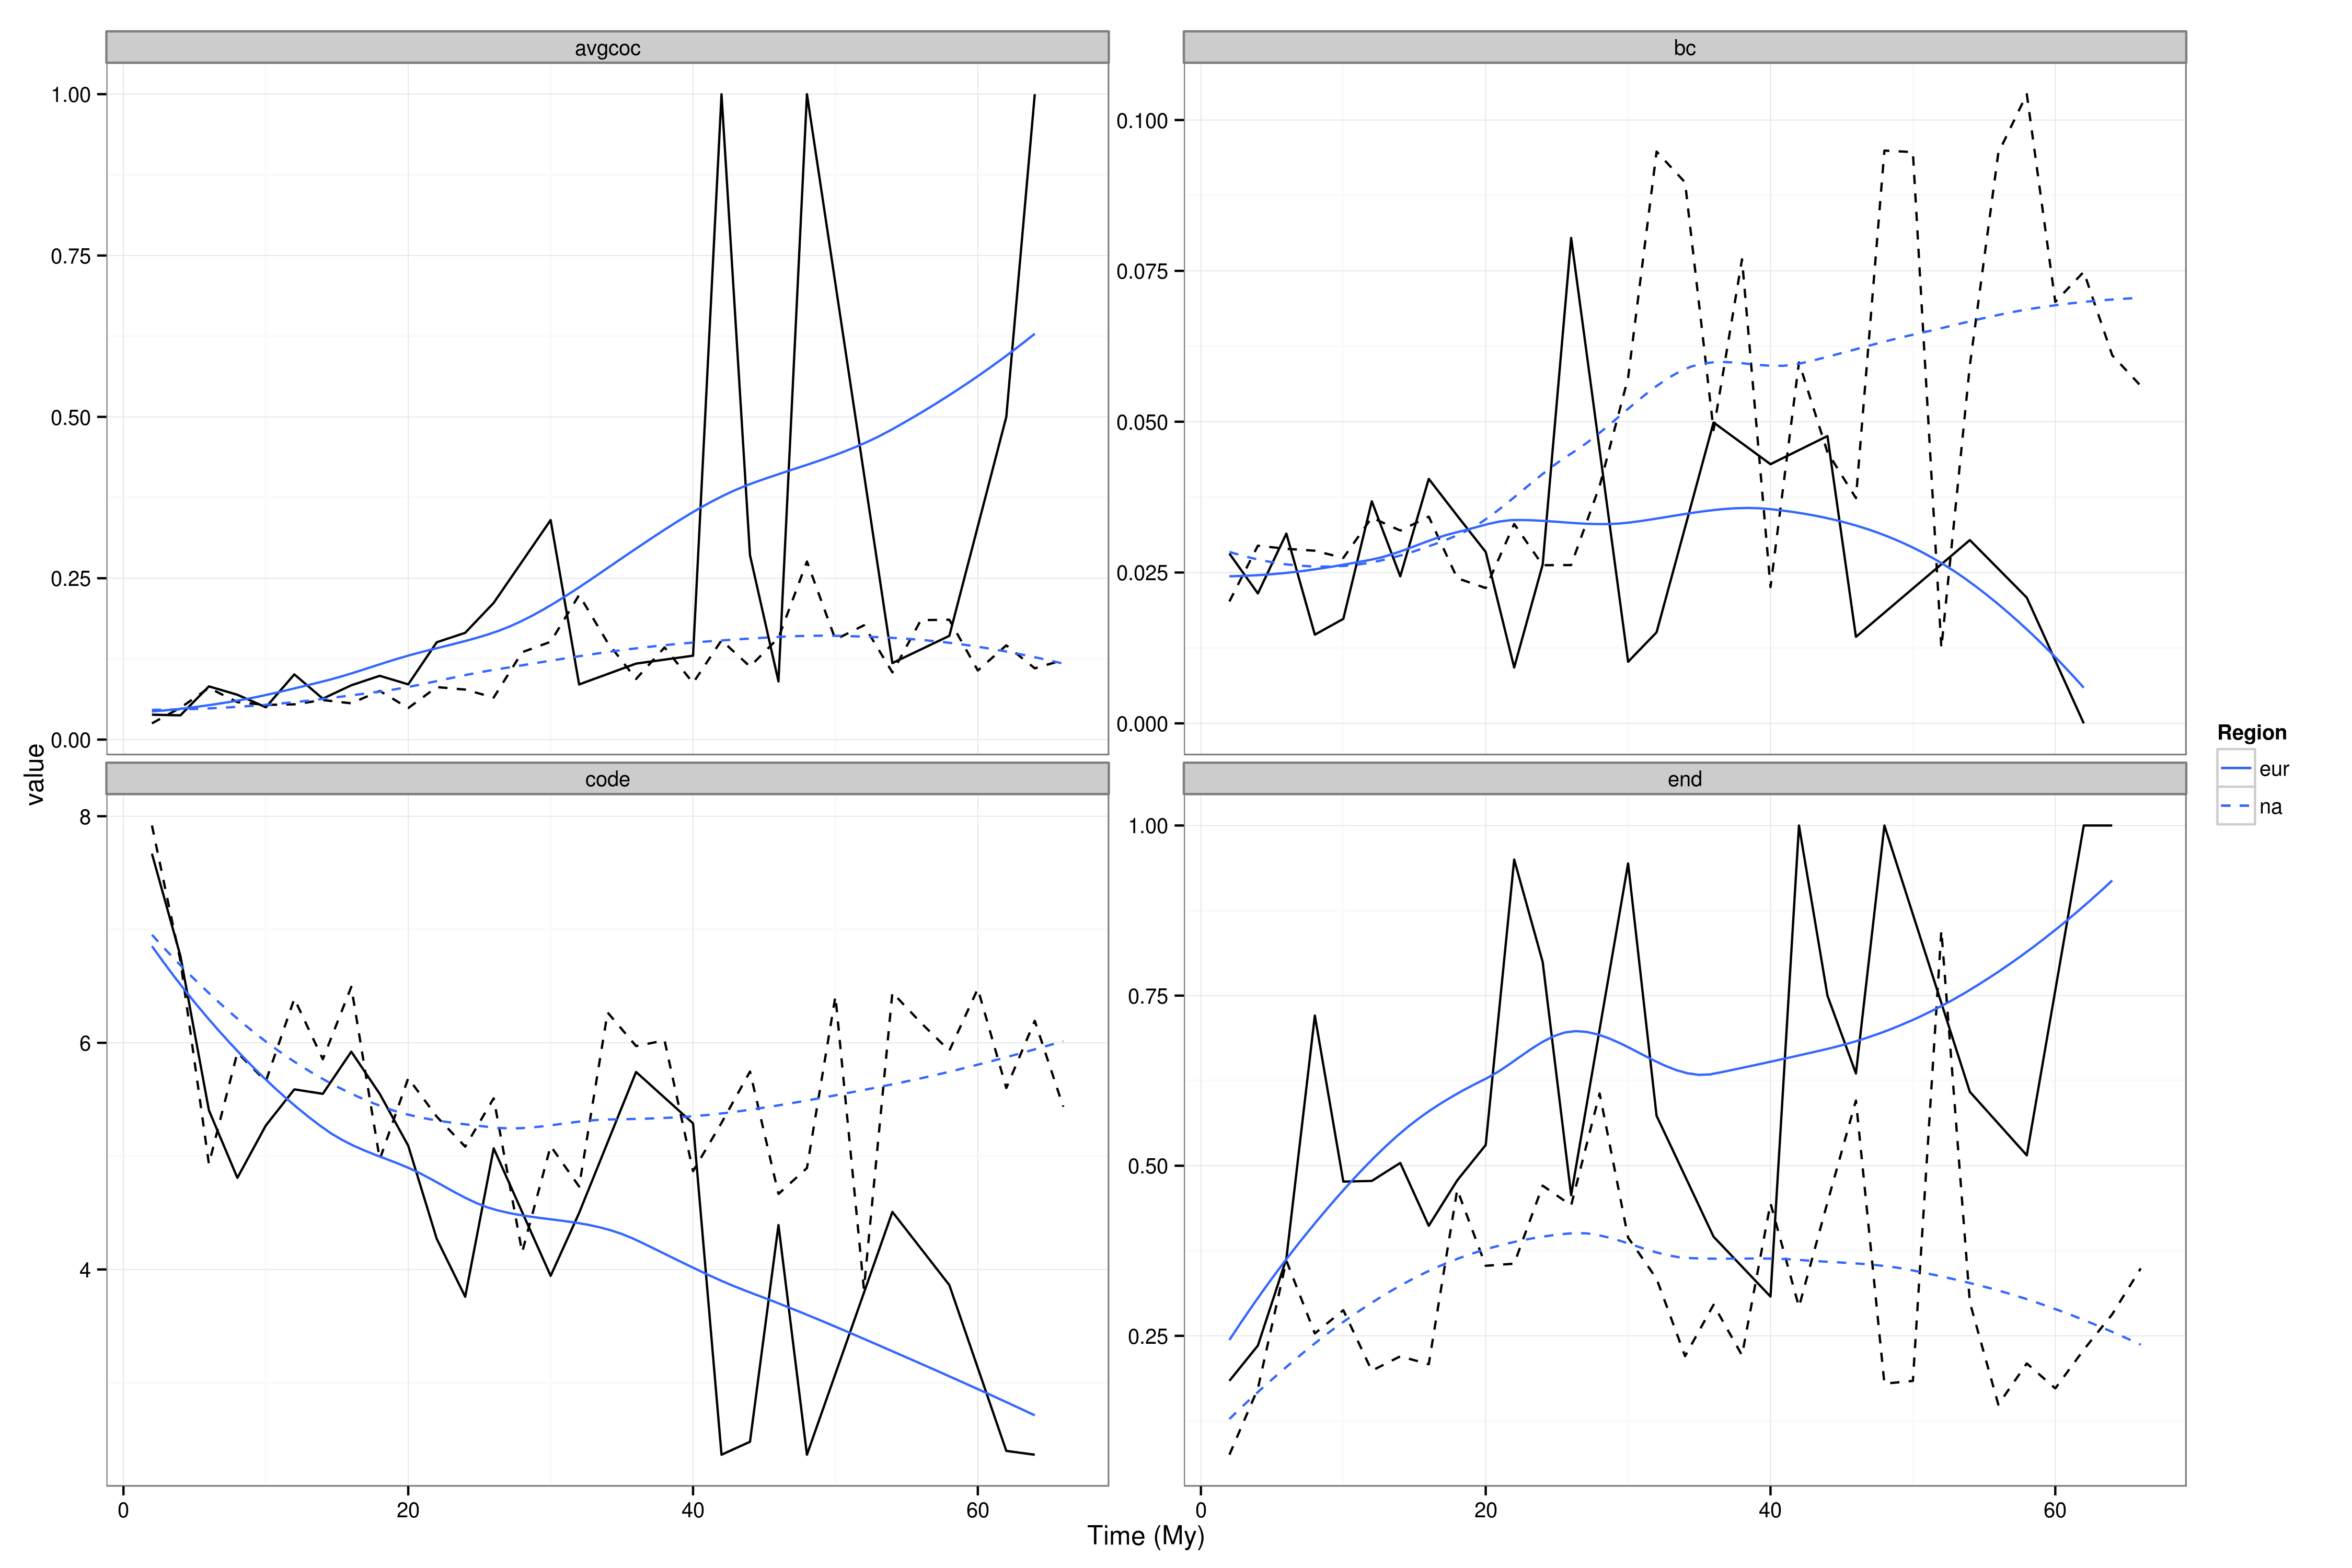
\includegraphics[height = 0.4\textheight, keepaspectratio = true]{figure/gen_bin}
  \end{center}
  \caption{Biogeographic network summary statistics for mammalian communities in North America (dashed line) and Europe (solid line). The summary statistics are, clockwise from top left: average relative occupancy (avgcoc), biogeographic connectedness (bc), average relative number of endemics (end), code length (code). Blue lines are generalized additive model smooths and are presented to illustrate the over all pattern of the two regions.} 
  \label{fig:mam_tot}
\end{figure}

While average relative occupancy remains relatively stationary for North America, there is a qualitative decrease in average relative occupancy in Europe until approximately the start of the Neogene (approximately 23 My). Average relative occupancy is a measure of how cosmopolitan any individual taxon is and the qualitative decrease in average relative occupancy in Europe over the entire Cenozoic indicates that the average taxon is becoming generally less cosmopolitan over time. In contrast, average relative occupancy in North America is qualitatively stationary over the entire Cenozoic and almost always lower than that observed for the European record. This means that, on average, North American taxa are present in very few localities at any given point in time.

Biogeographic connectedness is a measure of shared taxa between all localities, and higher values mean that more shared taxa then when there are lower values. Biogeographic connectedness of North American mammalian communities qualitatively decreases over the early Cenozoic until approximately the start of the Neogene. In Europe there is a qualitative rise in biogeographic connectedness in the first few million years of the Cenozoic, but afterwards remains relatively stationary. This may indicate that the average proportion of shared taxa remained qualitatively stationary. In comparison, North American remains stationary with a greater amount of shared taxa than Europe for the first half of the Cenozoic followed by a decrease and another plateau at the end of the Cenozoic.

In Europe, there is a over all qualitative decrease in average relative number of endemic taxa. North America, in contrast, has a qualitatively constant average relative number of endemics over the Cenozoic with a slight decrease in the Neogene. As discussed above, average relative number of endemics is a measure of relative uniqueness of localities. Qualitatively, North America retained approximately the same amount of site uniqueness through out the Cenozoic. In comparison, the pattern of the European record shows a qualitativly nonmonotonic decrease in locality uniqueness because of the decrease in average relative number of endemics.

The code length of European biogeographic networks increases qualitatively over the entire Cenozoic, while code length of North American networks remains relatively constant until the Neogene when there is a qualitative increase. Code length acts as a measure of general provinciality, with a high code length indicating little provincially between localities. Initial interpretation of these results indicates that North America maintains a stationary degree of provinciality while Europe has a qualitatively decreasing degree of provinciality. %The European results are consistent with the decrease in average relative number of endemics however is inconsistent with the decrease


\section{Ecology, survivorship, and fitness in Cenozoic mammals}

\textit{Questions:} 
How do ecological traits related to range size affect mammalian taxon duration? Is any single trait the best predictor of mammalian survivorship, or do multiple traits together best model taxon duration? Is climate an important factor in modeling mammalian taxon duration?

\textit{Background and Predictions:} 
As discussed above, dietary and locomotor categories are candidate constituent traits of range size. Additionally, body size is a classically cited constituent trait of range size \citep{Smith2004,Smith2008b,Damuth1981a,Damuth1979}. An organism of a certain body size has an associated energetic cost in order to maintain homeostasis, which in turn necessitates enough of the appropriate supply of prey items. Because of this, it is expected that larger organisms have higher energetic costs and thus a greater range size in order to obtain necessary resources \citep{Damuth1979,Brown1987,Damuth1979,Lyons2010}.

Mammalian herbivores and carnivores have been found to have a greater diversification rate than omnivores \citep{Price2012}. This analysis was global in scope, and based purely on extant taxa in a comparative phylogenetic context. Diversification rate can increase via either an increase in origination relative to extinction or a decrease in extinction relative to origination. Which of these two processes is occurring is (currently) impossible to determine from a phylogeny of only extant organisms \citep{Rabosky2010a} which means that analysis of the fossil record is necessary to estimate which scenario is most likely to have occurred. 

Depending on the continent, body size has been demonstrated to be related to extinction rate or not \citep{Tomiya2013,Liow2008}. By expanding to include a third continent, South America, I hope to elucidate how differences in taxonomic diversity at a continental level might affect body size mediated extinction rate. Additionally, I will be modeling body size as a continuous instead of binary variable.

\textit{Proposed research:}
To investigate the effect of ecological traits and climate change on survivorship, I plan to compare different models of trait based survival in order to best understand which factors are most important.

Survivorship analysis is the analysis of time-till-event data. In a paleontological context this is the time from origination (first appearance date; FAD) till extinction (last appearance date; LAD). Dietary category, locomotor category, and body size will be modeled as time-independent covariates of survival. The climate proxy \(\delta O^{18}\) oxygen curve \citep{Zachos2008} will be modeled as an ancillary time-dependent covariate. Also, constant versus time varying extinction rate will be estimated using different fundamental hazard models by comparing the fit of survival to various probability distributions.

%ADD IN MODELS. NEED TO READ MORE SURVIVAL BOOK.

While many previous analyses of survivorship are done using generic data \citep{Tomiya2013,Liow2008,Harnik2013}, there are potential biases in accurately modeling specific level processes using generic level data \citep{Raup1975,Sepkoski1975,Simpson2006,Raup1991a,VanValen1979}. There are important concerns regarding anagenesis, hierarchical selection, and taxa that did not go extinct in the time frame of interest \citep{Raup1975,VanValen1979,Simpson2006,Raup1991a}. Interestingly, the effect of incomplete sampling on estimation of survivorship curves appears rather minimal and uniform \citep{Sepkoski1975}. The problems involving taxa that did not go extinct have mostly been dealt with following advances in modeling right-censored and interval data \citep{Kleinbaum2005}.

In order to asses potential specific versus generic effects, I will estimate the difference between specific and generic mammalian survivorship models. Using an approach based on previous work to estimate specific origination and extinction rates from generic level survival curves \citep{Foote1988}, or a variant there of, I will measure the deviance between extinction rate estimated from the specific survivorship and the specific level extinction rates estimated from the analysis of the generic survivorship data. 

In addition to the above studies of mammalian survivorship, I also propose a simulation study to analyze effect of varying sampling probability and anagenesis on estimation of models of survivorship using \texttt{paleotree} \citep{Bapst2012a}. Phylogenies are frequently simulated as a time-homogeneous birth-death process, with a constant origination and extinction rate. The expected hazard function of survival is exponentially distrubuted with a time-constant rate parameter (\(\lambda\)). Sampling has been found to have minimal effect on inference of the survival function assuming biases are evenly distributed amongst taxa \citep{Sepkoski1975}, the affect of (cryptic) anagenesis is unknown. 

The data necessary to complete the empirical aspects of this study will be the same as for the above analysis of mammalian community connectedness.


\section{Permian brachiopods, extinction and environmental preference}

\textit{Questions:} In Australasian Permian brachiopods, do traits directly related to environmental preference relate to differential survival? Are certain traits more explanatory of survival than others? Does changing climate, habitat or substrate availability affect survival?

\textit{Background and Predictions:}
In brachiopods, three important ecological traits potentially involved in determining environmental preference are affixing strategy, substrate preference, and habitat preference. While larval mode is considered important in determining range size in marine invertebrates \citep{Jablonski2006a,Jablonski1983}, this does not preserve in brachiopods and thus cannot be used to directly model survivorship \citep{Jablonski1983}. Substrate preference is statement of the chemical and physical processes affecting the environment and acts as a limiting factor on the range of possible environments in which an organism can optimally survive. This then limits the possible geographic extent of a taxon. Substrate selection is mitigated via larval chemosensory abilities and thus may be a weak proxy for larval dispersal ability \citep{Jablonski2006a,Jablonski1983}. 

Affixing strategy and habitat preference relate to range size by means of limiting the possible geographic extent of a taxon. Affixing strategy is the manner by with an individual interfaces with the substrate. Different strategies are optimal for certain environmental conditions such as flow speed or mud depth \citep{Alexander1977,LaBarbera1978,LaBarbera1981}. Because brachiopods are obligate filter feeders, flow speed and environmental energetics are important in prey capture and individual survival. Thus, the availability of optimal environments becomes a limiting factor on the possible geographic extent of a taxon. Habitat preference is a statement of the suitability of an environment and the accompanying environmental energy level and acts as a limit on the possible geographic extent of a taxon. 

The three principle ways of classifying affixing strategies are pedunculate, reclining, and cementing. During the Permian, pedunculate taxa tend to be associated with shallow on-shore environments while reclining taxa are associated with deep off-shore environments \citep{Clapham2007}. However, this association is weak as most assemblages are composed of a heterogeneous mix of taxa \citep{Clapham2007}. Previous analysis of brachiopod durations indicated that affixing strategy is associated with differential longevity \citep{Alexander1977}. Among endemic taxa, reclining taxa have longer durations than all other affixing strategies. In contrast, among cosmopolitan taxa, pedunculate and cementing taxa had longer durations than all other taxa. 

The three principle classifications of substrate affinity are carbonate, clastic, or mixed. These are descriptions of the lithology of the sites at which the taxa are predominately found \citep{Foote2006,Anderson2011a,Nurnberg2013a,Kiessling2007a,Miller2001}. The Pharenozoic is characterized by an overall decline in carbonates relative to clastics \citep{Foote2006,Miller2001}. Because of this, it is expected that taxa with clasitic or mixed affinities will have greater durations than taxa associated with carbonate substrates. % Brachiopods are mixed slash switchers CARL AND MELANIE'S UNPUBLISHED WORK.

The primary ways of classifying habitat preference are on-shore, off-shore, or mixed. Habitat preference has been the focus of a great deal of research in terms of explaining global diversity dynamics \citep{Sepkoski1991,Kiessling2007a,Bottjer1988,Jablonski1991,Jablonski1983b}. Importantly, habitat preference is related to sea-level rise and fall and the availability of that habitat with changing environment. On-shore environments have declined in areal extent over the Pharenozoic \citep{Peters2008}. Because of this decrease in areal extent, the expectation would be that taxa predominately associated with on-shore habitats would have overall lower durations than taxa associated with off-shore habitats or mixed preference. 

An important consideration is that taxonomic survival might not be linked to single environments \textit{per se}, but the variability of environments \citep{Foote2013,Heim2011,Liow2007b}. This adaptation to variable environments has been found to relate strongly with survival past origination \citep{Foote2013}. In this case, it would be expected then that taxa with mixed preferences for both substrate and habitat would have potentially longer durations than taxa with single preferences. This makes logical sense as it would mean that a taxon's potential geographic extent is not expressly limited by either of these two traits and thus decreasing expected extinction rate due to large range size \citep{Jablonski1986,Harnik2013,Nurnberg2013a,Jablonski2003,Roy2009c}. 

During the Permian there was a shift from an ``ice house'' to a ``hot house'' world \citep{Fielding2006,Birgenheier2010,Jones2006,Powell2007} which could be expected to have some effect on brachiopod survivorship. Taxa in Australia are of particular interest because of their proximity to the south pole during the Permian and the repeated glacial activity in the region \citep{Fielding2006,Birgenheier2010,Jones2006}. According to \citet{Olszewski2004}, sea-level and climate change do not wholly explain the ecological dynamics experienced by brachiopods in the Permian of Texas. The prediction then is that the best model of brachiopod survivorship will have to have some biotic component such as affixing strategy or substrate preference. Climate being a predictor in the best model of survivorship is less clear cut and necessary to determine empirically.


\textit{Proposed research:}
I propose to a survival analysis approach similar to that described above to estimate the differential survivorship of Permian brachiopods. I restrict this analysis to Australiasia because it represents a relatively continually sampled and well worked area that preserves the majority of the entire Permian \citep{Clapham2012,Clapham2008a,Waterhouse1987,Archbold1995}. In this analysis, the time-independent covariates are substrate preference, affixing strategy, and habitat preference. Climate will be modeled as either an ancillary Heaviside function or a time-dependent covariate depending on the quality of the Permian isotope record. Additionally, as in the mammalian survivorship analysis described above, the age dependence of brachiopod extinction rates will be estimated using different fundamental hazard models by comparing the fit various probability distributions to survival.

Permian brachiopod occurrence information is available via the PBDB and is primarily based on the work of Clapham \citep{Clapham2006,Clapham2008a,Clapham2007a,Clapham2012,Clapham2007} and \citet{Waterhouse1987}.


\textit{Preliminary results}
Preliminary analysis of brachiopod survivorship based on substrate affinity and habitat preference. Depositional environment of all occurrences were classified into one of the three substrate affinity categories following \citet{Foote2006} while paleoenvironmental setting of all occurrences were classified into one of the three habitat preferences following \citet{Kiessling2007}. Both of these traits were assigned using the approach of \citet{Simpson2009} where trait value is determined as the posterior probability of the occurrence ratio in comparison to the all occurrences during the duration of that taxon. Assignment probability (\(P(H_{1}|E)\)) was calculated as
\begin{equation}
  P(H_{1}|E) = \frac{P(E|H_{1})P(H_{1})}{P(E|H_{1})P(H_{1}) + P(E|H_{2})P(H_{2})}
  %\label{eq:aff}
\end{equation}
where \(P(H_{1})\) and \(P(H_{2})\) were prior probabilities of assignment while \(P(E|H_{1})\) and \(P(E|H_{2})\) were conditional, binomial probabilities. 

For substrate affinity \(P(H_{1}) = P(H_{2}) = 0.5\) and if \(P(H_{1}|E) > \frac{2}{3}\) then the taxon was considered of carbonate affinity while if \(P(H_{1}|E) < \frac{1}{3}\) then the taxon was considered to have a clastic affinity. Otherwise, the taxon was considered to have no or mixed affinity. In the case of habitat affinity, the posterior probability for each habitat (inshore, offshore, none) was calculated with \(P(H_{1}) = \frac{1}{3}\) and \(P(H_{2}) = \frac{2}{3}\) and the preference with maximum of the three posterior probabilities was the assignment.

Preliminary parametric model fitting with both exponential and Weibull hazard functions and either or both trait indicated that the best fit model based on comparison of AICc scores \citep{Hurvich1989,Akaike1974,Burnham2002a} was the model with substrate affinity as the sole predictor and a Weibull hazard function. This model is illustrated below (Fig. \ref{subfig:aff_surv}). While this model is the preliminarily best model of survivorship, the model with both substrate affinity and habitat preference as additive effects and a Weibull hazard function is almost as good a model of survival (\(\Delta\)AICc \(\approx 0.9\)). Additionally, as illustrated by the difference between the nonparametric Kaplan-Meier survival curves and the predictions of the parametric model of survival (Fig. \ref{subfig:aff_surv}) and there is room for improvement in model specification. 

\begin{figure}[ht]
%  \begin{center}
    \begin{subfigure}[b]{0.5\textwidth}
      \caption{}
      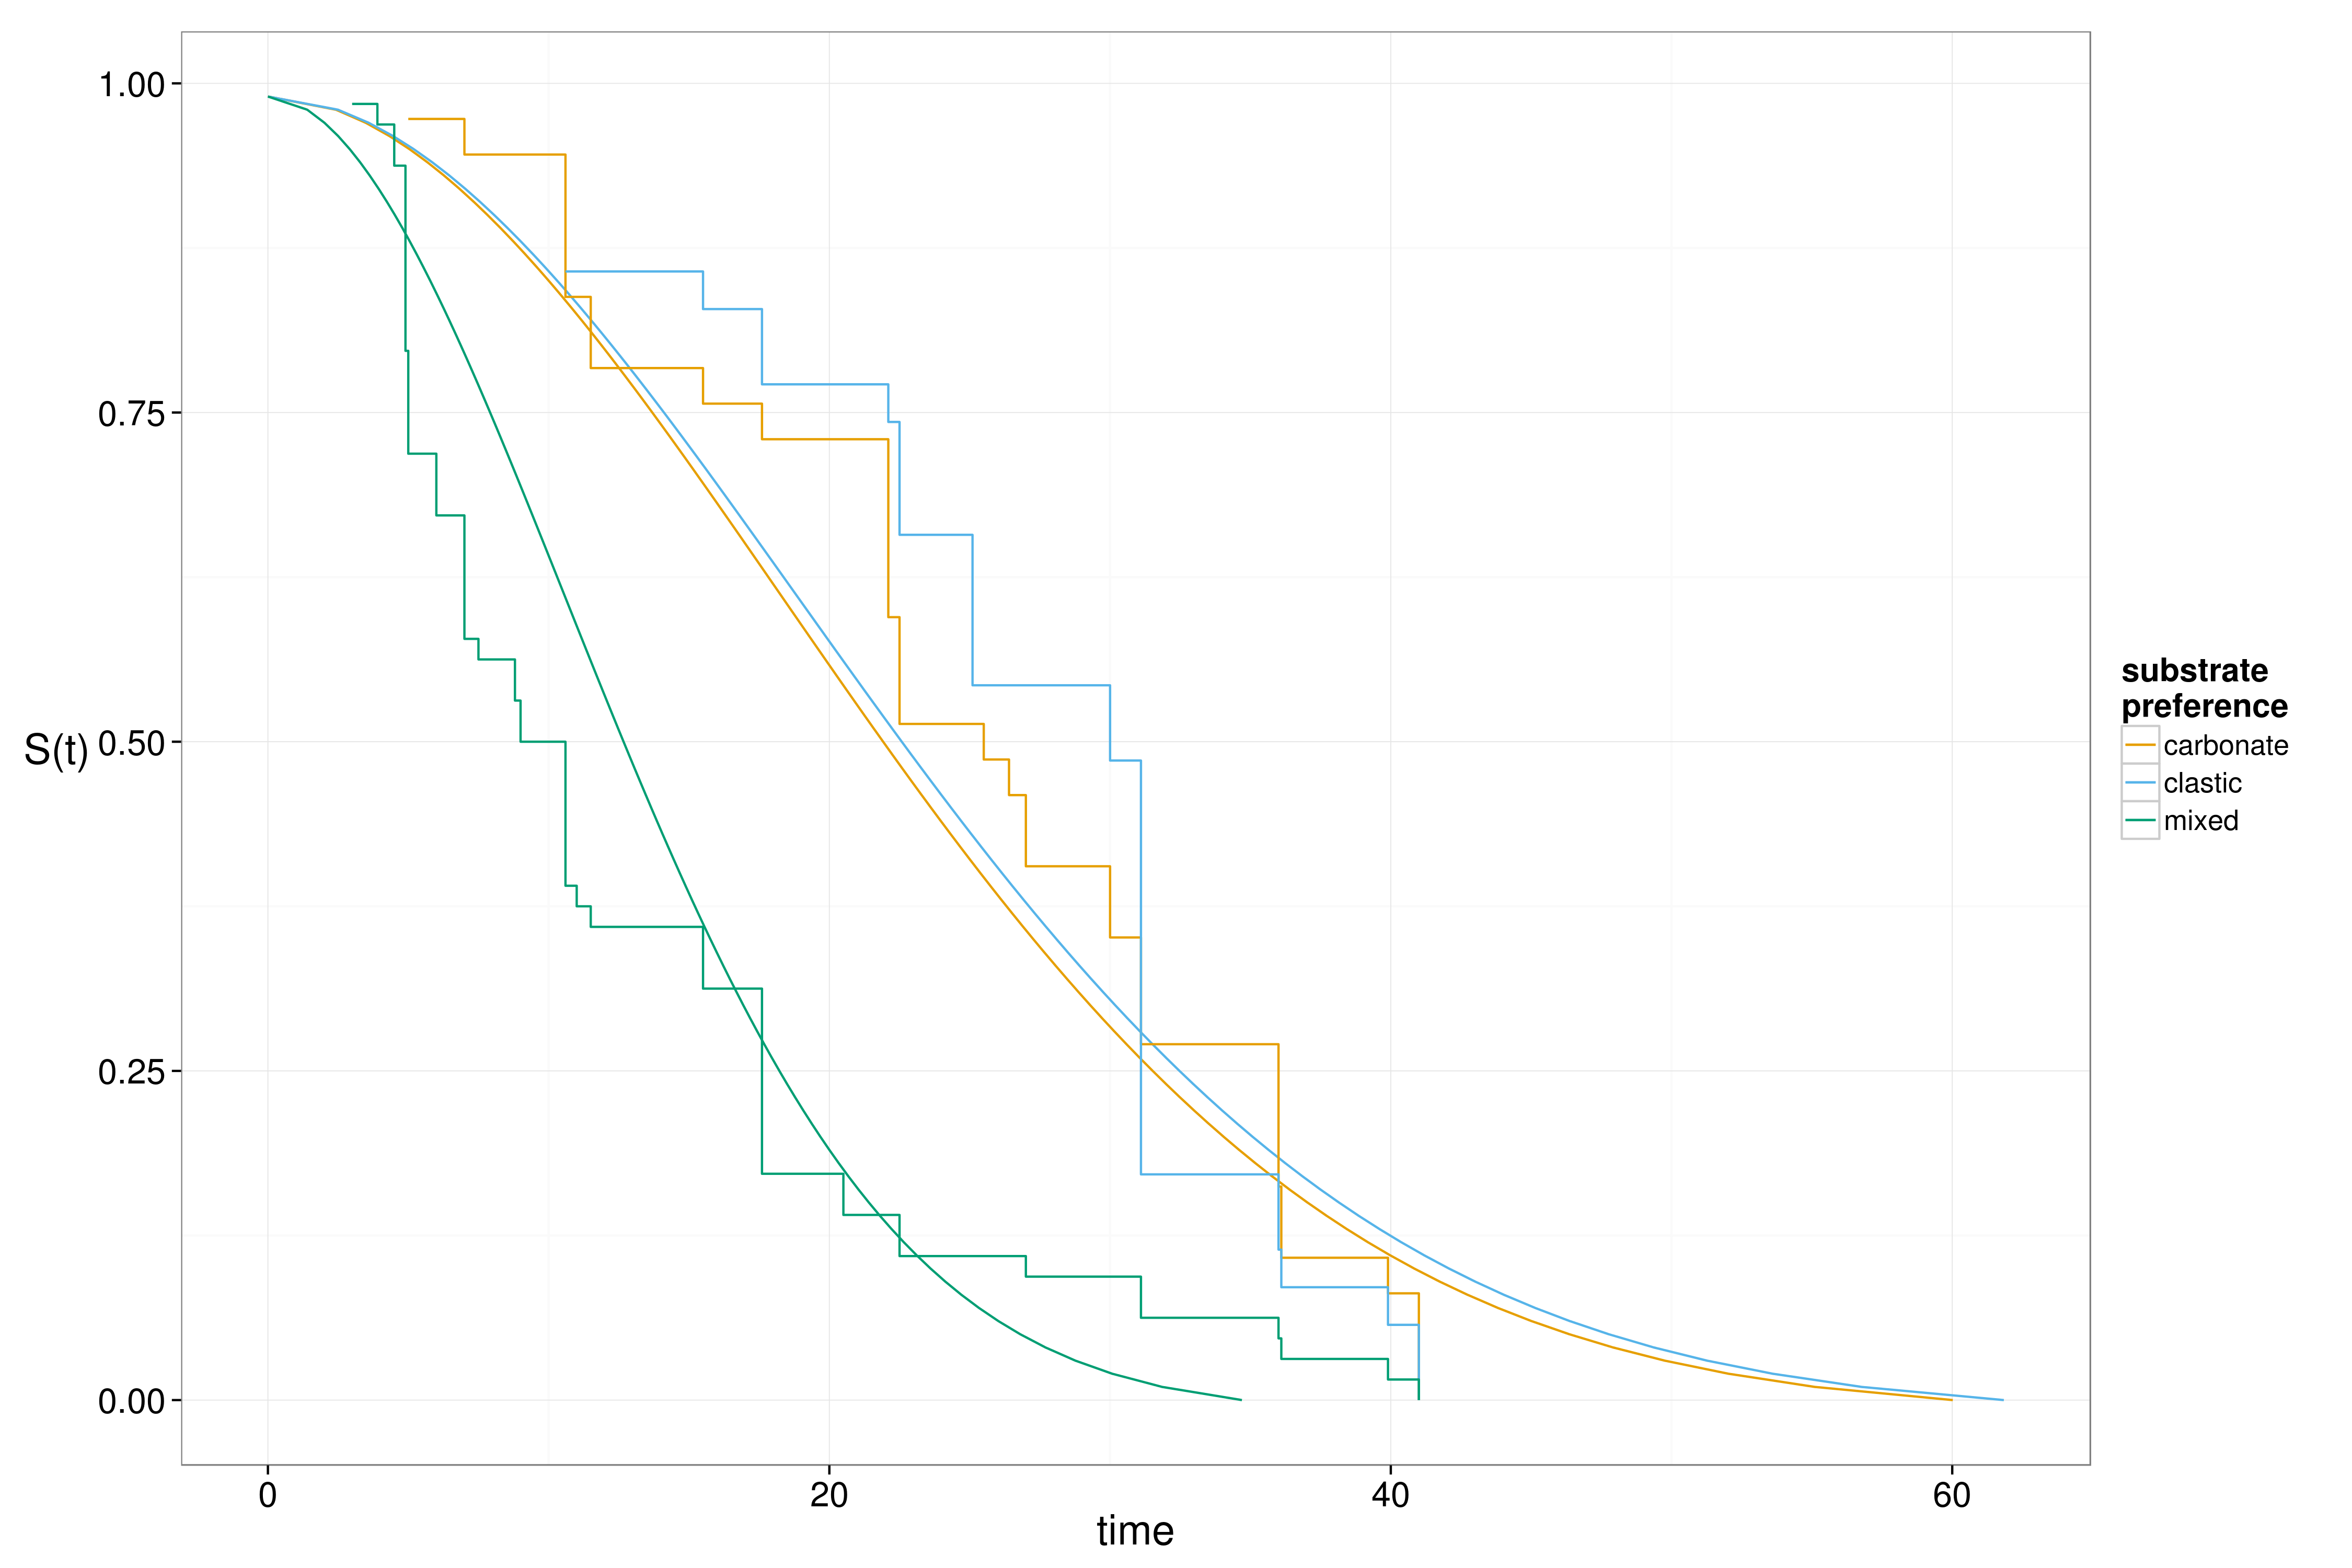
\includegraphics[height = 0.4\textheight, keepaspectratio = true]{figure/aff}
      \label{subfig:aff_surv}
    \end{subfigure}
    \begin{subfigure}[b]{0.5\textwidth}
      \caption{}
      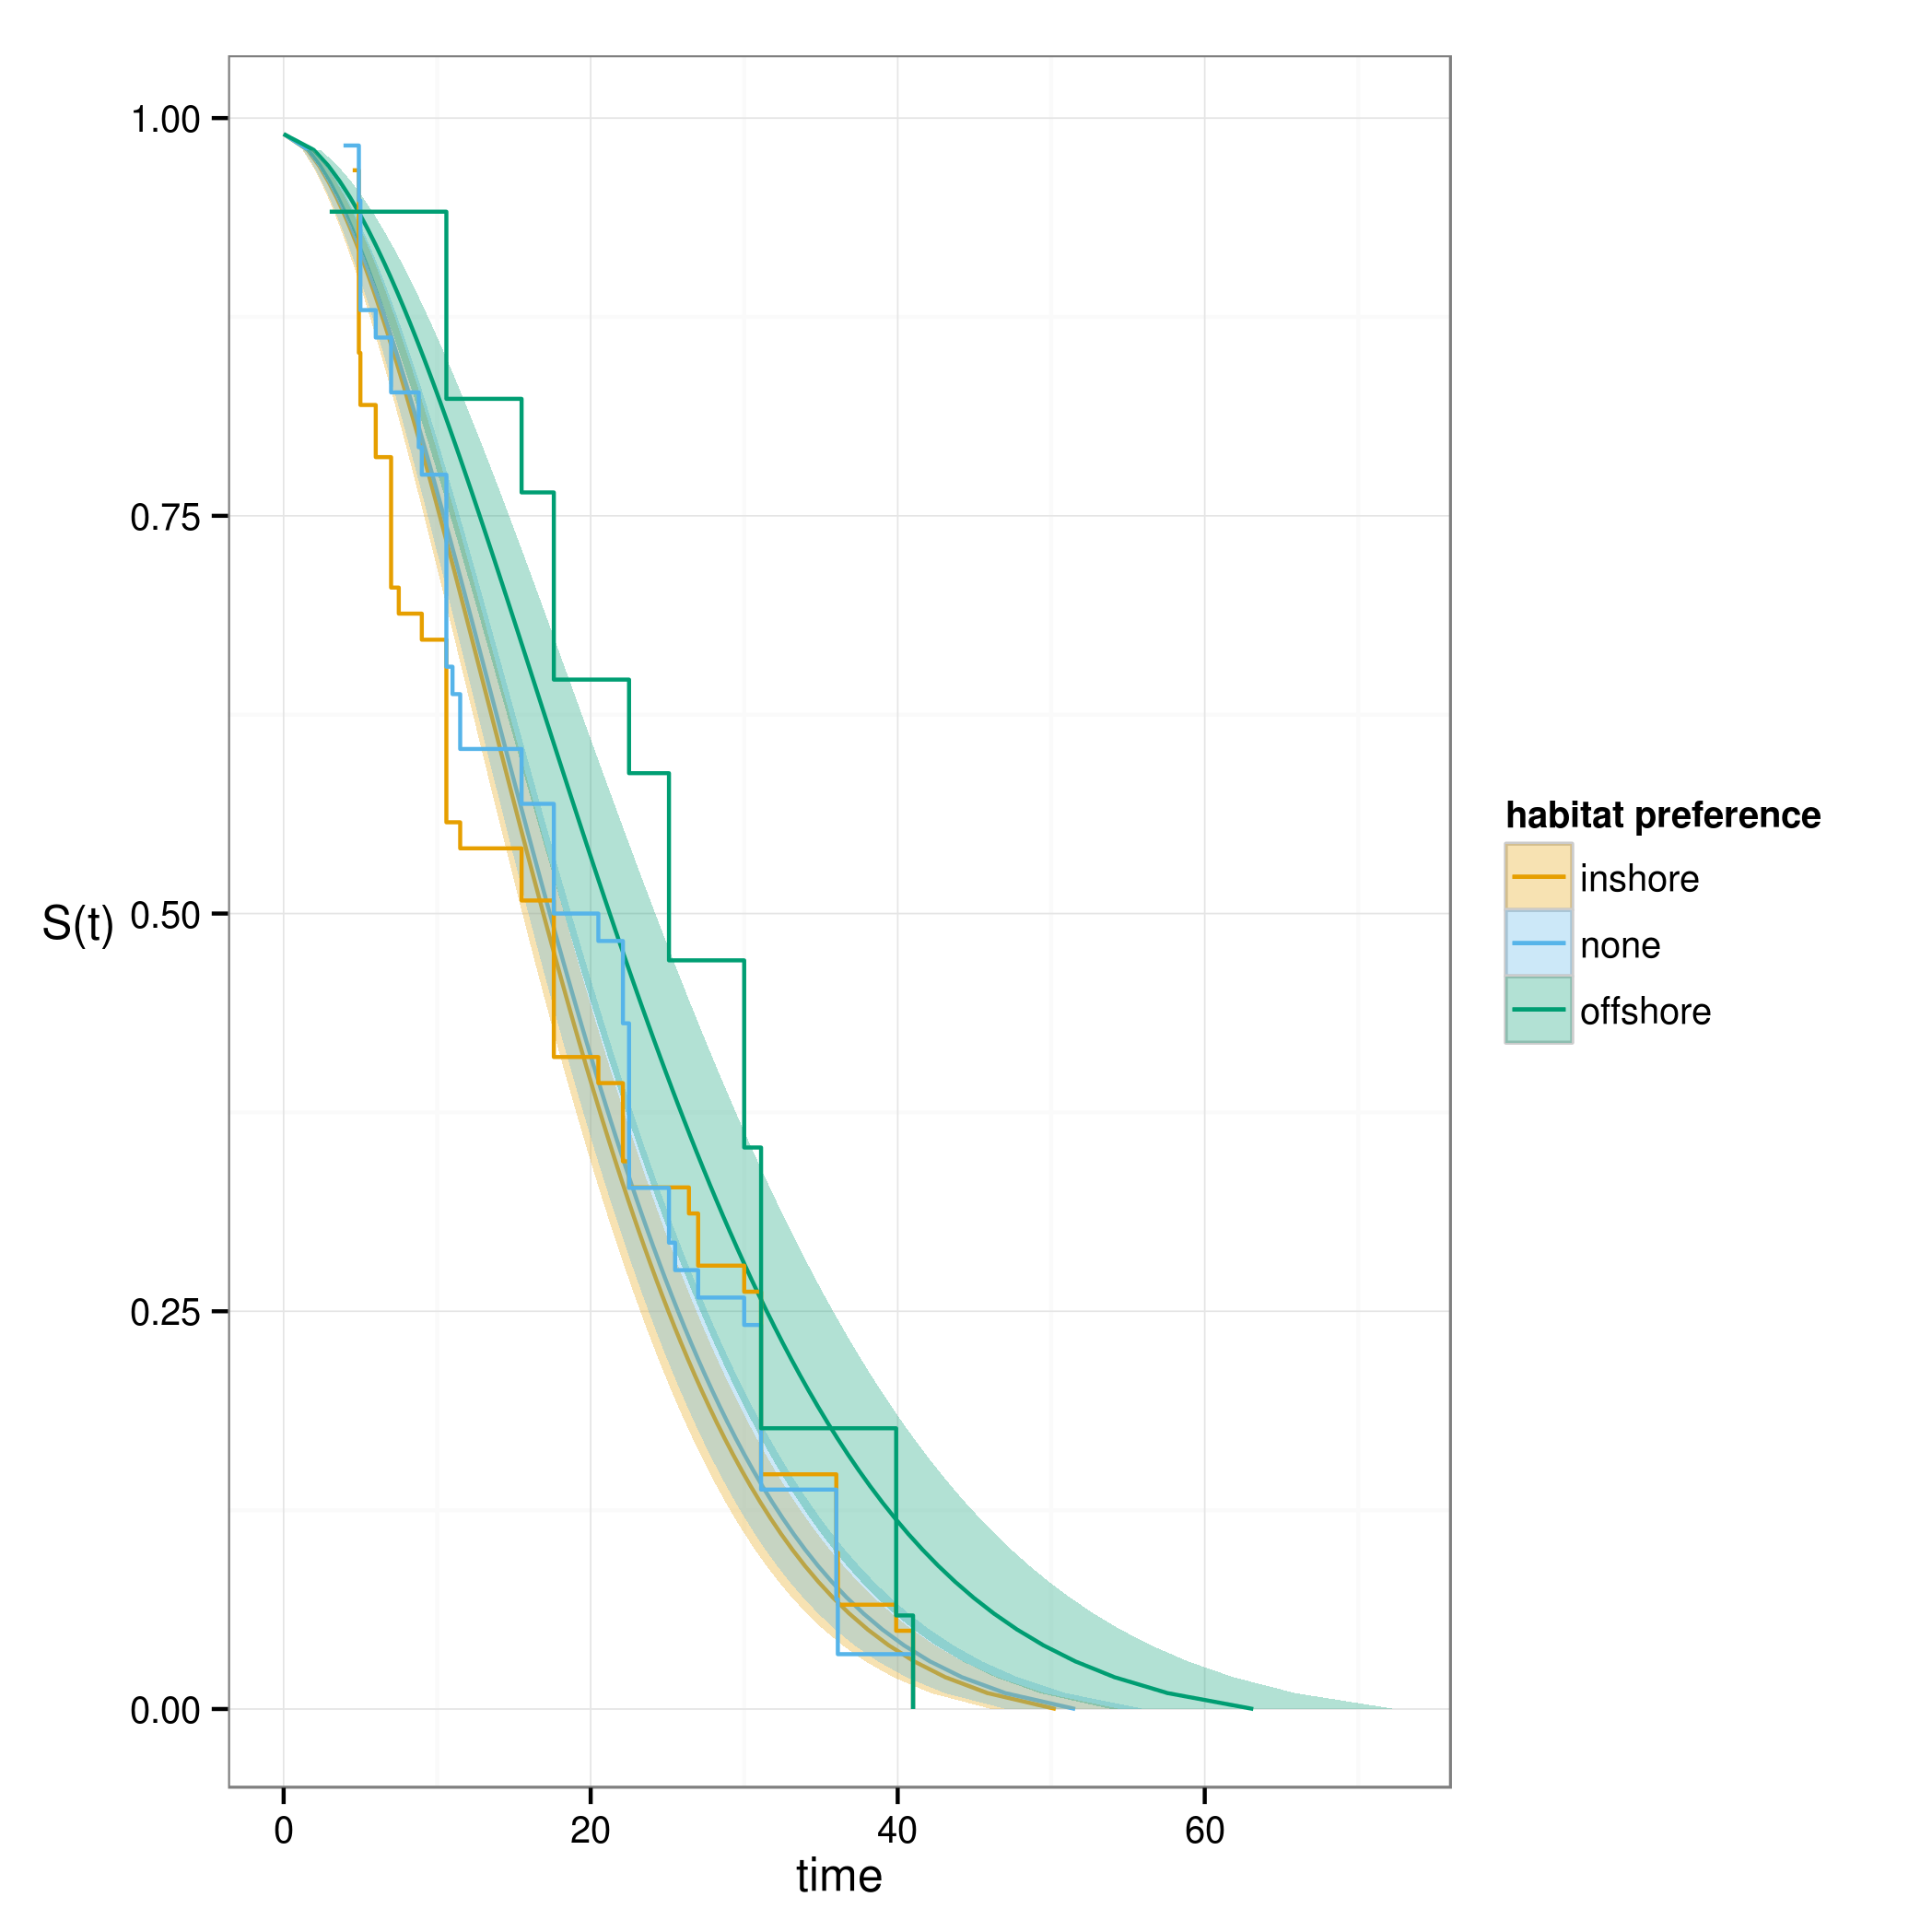
\includegraphics[height = 0.4\textheight, keepaspectratio = true]{figure/env}
      \label{subfig:env_surv}
    \end{subfigure}
%  \end{center}
    \caption{Survivorship curves of Australasian Permian brachiopod genera based on substrate affinity (\subref{subfig:aff_surv}) and habitat preference (\subref{subfig:env_surv}). The three stepwise functions are nonparametric Kaplan-Meier survival curves for each of the three substrate affinities. The three smooth lines are the predicted survivorship probabilities for taxon of the given age from the parametric model of generic survivorship and illustrated standard errors of the prediction.}
  \label{fig:brach_surv}
\end{figure}

The AICc best survival modeling has substrate affinity as the sole predictor and the response modeled as a Weibull distribution. Importantly, the shape parameter (\(k\)) of the Weibull distribution is estimated to be approximately 1.3. Values of \(k\) that are greater than 1 means that failure (extinction) rate increases with time, which may mean that an age-independent extinction rate is inappropriate when modeling generic level diversification in brachiopods. % contra Foote and certainly contra Van Valen?

For brachiopods split but substrate affinity (Fig. \ref{subfig:aff_surv}), survival probability of low duration (time) values are higher in both carbonate and clastic lowest in taxa with mixed durations. In comparison, the survival probabilities of high duration (time) values is highest in carbonates and very low in both clastic and mixed duration taxa. There is a noticeable deviance between the estimated survival function and the nonparametric curve for taxa with clastic affinities at both the short durations and long durations, underestimating and overestimating respectively. Otherwise, the estimated survival functions are fairly good fits for the data. 

For brachiopods split by environmental affinity and survival modeled as a Weibull distribution is not a as good model of survival, with an approximate \(\Delta\)AICc of 16.8 between this model and the previous model. There is a great degree of deviance between the nonparametric Kaplan-Meier curves and the model predictions. Additionally, this model is not significantly different from the model with only an intercept (\(\chi^{2} = 1.99\), \(df = 2\), \(p = 0.37\)). This means, preliminarily, that habitat preference alone makes no difference in generic level extinction rate.

Further refinements to these models include modeling survival using other distributions of survival such as a log-normal distribution. Additionally the inclusion of affixing strategy as a predictor will increase the understanding of the biology underlying brachiopod generic survival based on organismal traits.

\section{Summary of proposed research}
One of the most important questions in (paleo)biology is why do certain species go extinct while others do not? Elucidating what interactions, or traits governing interactions, are important when estimating survival is then extremely important and a fundamental concern of evolutionary paleoecology. While the species level property of range size is continually found to be an extremely vital for both origination and extinction \citep{Roy2009c,Foote2013,Jablonski2003,Jablonski1987,Harnik2013}, which of the candidate constituent lower level traits are necessary to ``form'' range size remains more nebulous and is frequently framed as which traits in addition to range size \citep{Foote2013,Harnik2011,Nurnberg2013a}. Related to this is the general question of how climate change impacts diversity dynamics \citep{Barnosky2001a,Alroy2000g,Figueirido2012,Olszewski2004}. Here I compare the impact of various constituent traits of range size on both community connectedness and survival. The former is a discussion of the range and limitations of possible biotic--biotic interactors and the later is a discussion of what ecological traits, either alone or in concert, best model time from origination till extinction. By comparing two distantly related clades, mammals and brachiopods, the hope is to determine how necessary discussion of ``emergent'' properties is and how ecological traits may interact to increase the survival of a taxon.


\clearpage
\section{Timeline}

Spring/Summer 2014
\begin{itemize}
  \item Evolution Meeting: preliminary brachiopod survival results
  \item South American fossil mammal data from Field Museum of Natural History collections
\end{itemize}

Fall 2014/Winter 2015
\begin{itemize}
  \item GSA: survivorship simulation for anagenesis and sampling
  \item Doctoral Dissertation Improvement Grant
\end{itemize}

Spring/Summer 2015
\begin{itemize}
  \item Evolution Meeting: mammalian survivorship analysis for North America and Europe
  \item South American fossil mammal data from American Museum of Natural History collections
  \item write and submit survivorship simulation paper
\end{itemize}

Fall 2015/Winter 2016
\begin{itemize}
  \item SVP or GSA: mammalian biogeographic connectedness
  \item write and submit mammal connectedness paper
\end{itemize}

Spring/Summer 2016
\begin{itemize}
  \item Evolution Meeting: brachiopod survival analysis results
  \item write and submit brachiopod survival paper
\end{itemize}

Fall 2016/Winter 2017
\begin{itemize}
  \item SVP or GSA: mammalian survivorship analysis
  \item write and submit mammal survival paper
\end{itemize}

Spring/Summer 2017
\begin{itemize}
  \item Evolution Meeting
  \item write and submit review/philosophy paper
  \item \textbf{Defend}
\end{itemize}



\clearpage
\bibliographystyle{abbrvnat}
\bibliography{proposal}

\end{document}
